\section{system design}
We have developed an Android application, DirectionDetector, which provides an interface to start/stop the angle estimation process. The application interface displays the estimated angle with respect to the camcorder microphone (the one closer to the camera). Figure ~\ref{fig:screenshot} [insert a figure number here] shows the screenshot of the application. [?????? add a figure that shows the way of angle measurement visually].

\begin{figure}
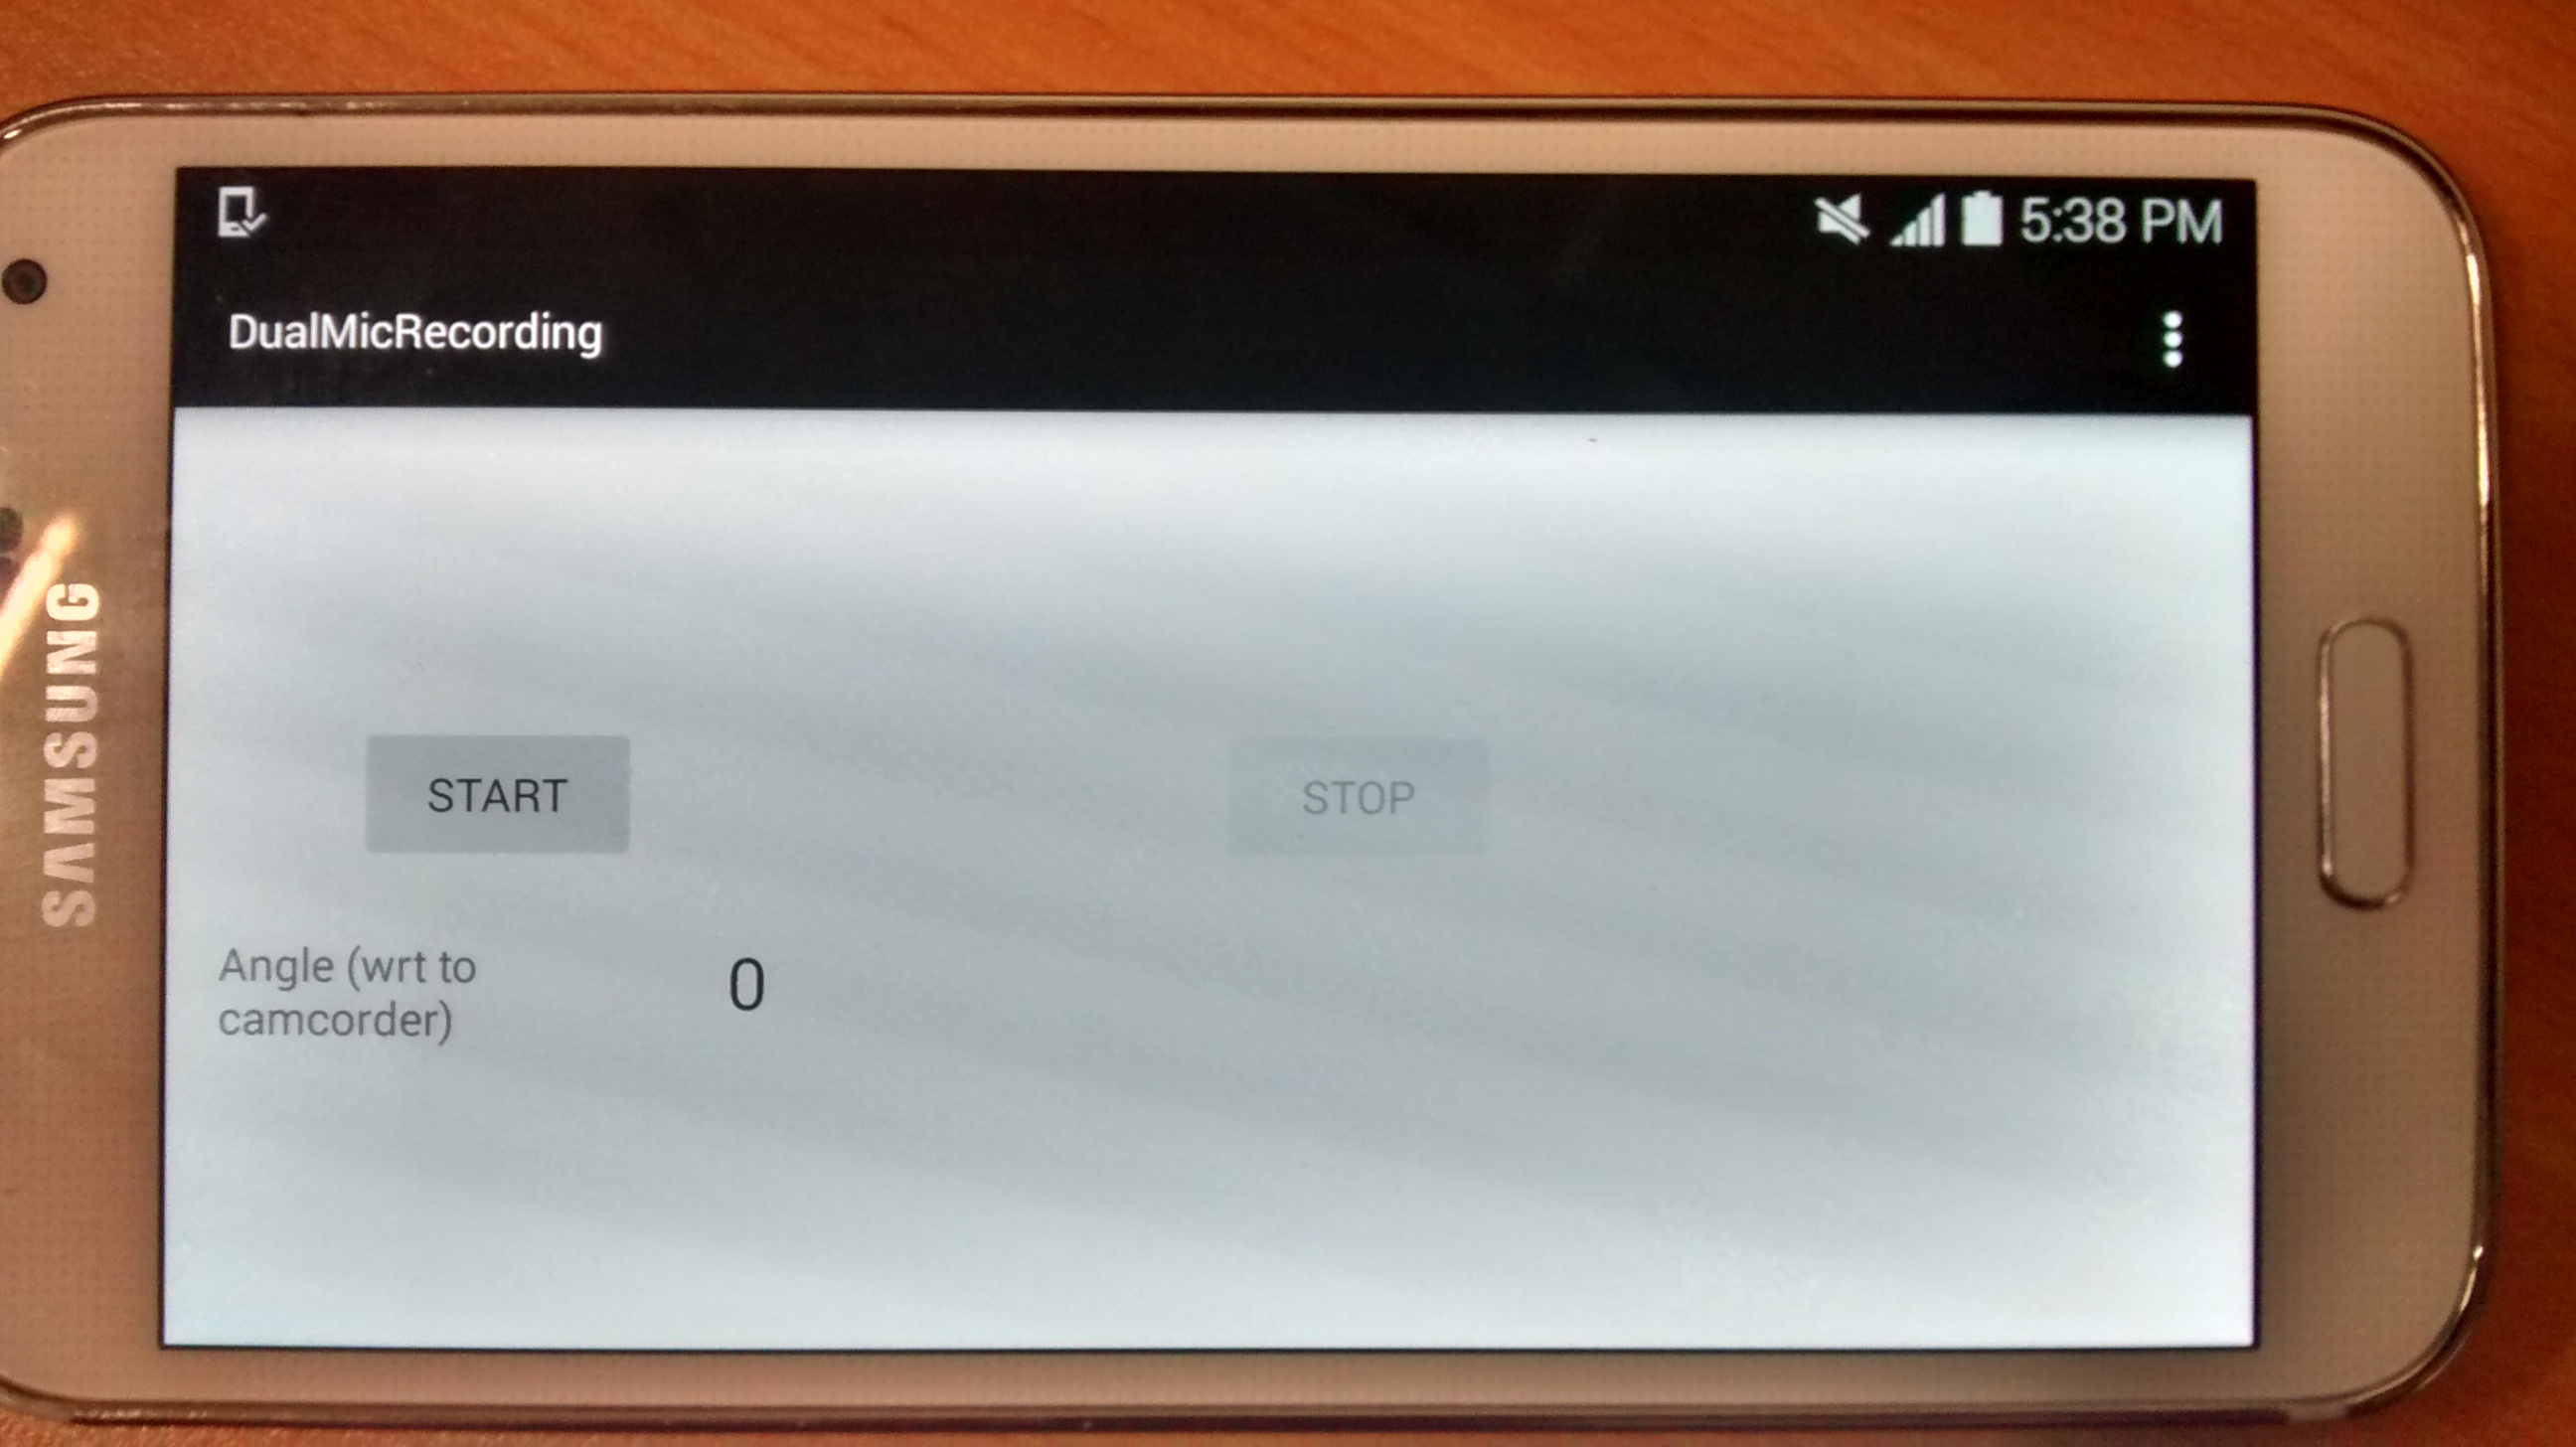
\includegraphics[width=90mm, height=60mm]{figures/screenshot.jpg}
\caption{Android Application Screenshot}
\label{fig:screenshot}
\end{figure}


\begin{figure}
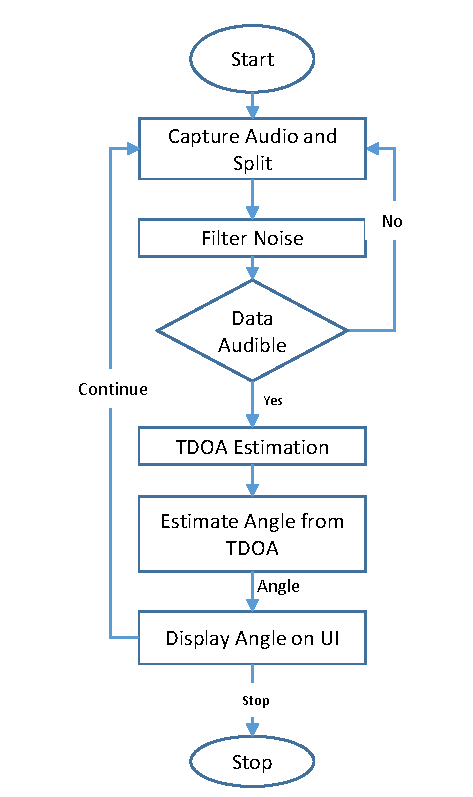
\includegraphics[width=80mm, height=100mm]{figures/flowchart.pdf}
%\includesvg{figures/flow_chart.svg}
\caption{Flow Chart of Angle Estimation}
\label{fig:flowChart}
\end{figure}

The flow chart in Figure ~\ref{flowChart} represents the steps involved in angle estimation. Once the user starts the detection process, by clicking on start button on application interface, the application start capturing sound samples from both the microphones i.e. camcorder and mic. The sampling rate can be varied from 8000 HZ to 44100 HZ. For our experiments, we used 44100 HZ because Android guarantees to support this sampling rate at all devices and also using higher frequency provides a better estimate. Each step of flow chart is explained below.
\subsection{Capture Audio \& Split }
When recording audio in stereo mode, Android puts captured audio frames from both the microphones in one single buffer. Frames at even indices belong to one channel and those at odd indices belong to another channel. For processing, the application can read data from this system buffer and then split frames for both channels. In our analysis we read 4096 samples at a time from Android buffer and before proceeding further, we split this array into two different vectors, one for \textit{camcorder} data and other for the \textit{mic} data. Elements of these arrays are called frames of audio data. Individual frames are processed for angle estimation. 

\subsection{Noise filter}
Since the environment may have some ambient noises, so before estimating angle for captured samples, we filter the possible noise. We compute root mean square value of sound magnitude. If this magnitude is lower than a certain threshold, then these samples are not used for angle estimation and rather discarded. Samples with root mean square value above the threshold are passed to the angle estimation module. Also, some smartphones might have an inbuilt noise suppressor module, so on devices with that capability, we use noise suppressor module together with our noise filter to filter samples in better way.

\subsection{TDOA estimation}
The objective of this step is to estimate TDOA of both signals. The time difference might arise because microphones might be at different distances from the sound source. Given two audio signals,   cross-correlation can be used for lag estimation. The idea behind this approach is that two similar audio signals would have maximum correlation. Sum of the products of frames in camcorder and mic vectors will be maximum when both signals are similar. So, given camcorder and mic data array, we shift the frames of mic array and compute sum of products of frames of both arrays for this shift. Each shift corresponds to a lag in terms of delay in number of audio frames with respect to camcorder. For example, we start by left shifting elements of mic array by N. For this shift, sum of products of elements of camcorder and mic array is computed and  stored. This represents correlation value corresponding to lag equal to -N . This negative lag means that mic samples lag behind camcorder samples by N number of frames. Similarly, we compute correlation value for left shift equal to N-1 and store it. This process is carried on for N times for left shift followed by N times for right shift. We also compute sum of products for 0 lag. The value of N is dependent on distance between two microphones and the sampling frequency. The formula for N is given below.

\begin{gather*}
N =  \frac{d} {v} *S
\end{gather*}

Here, d represents the distance between two microphones, v is sound velocity in air (343 m/s) and S is sampling frequency. From all these correlation values for different lags, we pick the maximum value and record the lag corresponding to that value. This lag value is actually lag in terms of number of frames, so we divide it with sampling frequency to calculate TDOA which represents difference in time-of-arrival in seconds.

For value of d equals 0.14 meter and S equals 44100 Hz, the value of N comes out to be 18. So, we can shift our signal vectors from -18 to +18 resulting in 37 possible values of lag. Since each lag value can be mapped to an angle of arrival, so this technique can estimate 37 different angles in 0 to 180 degrees.


\subsection{Compute angle from TDOA}
Once we have TDOA, we estimate angle of arrival from it. The angle of arrival derivation looks like as shown in Figure ~\ref{fig:aoaDerivation}. In this figure, the sound source lies somewhere in first quadrant and the inclined straight lines represents sound waves coming from the source. Left red cross corresponds to camcorder and right cross to mic of smartphone. Value of d represents the distance between camcorder and mic measured in meters, $d_T$ represents difference in distance travelled by each audio frame to reach both the microphones, $v_2$ represents sound velocity in air and $\theta$ represents the angle of arrival with respect to camcorder of the smartphone. After estimating TDOA in previous step, we can compute  $d_T$ using velocity of sound in air (343m/s). Once all these values are computed then $\theta$ can be computed by following formula.
\begin{gather*}
\theta = \cos^{-1}(\frac{v_2 * TDOA}{d})
\end{gather*}


Value of angle from this equation can vary from 0 to 90 degree because of right angle triangle. So, in order to estimate angle of arrival for sound source in second quadrant, we use sign of lag. If lag value is negative then the sound source is in second quadrant (closer to camcorder) and if it is positive, then sound source lies in first quadrant (closer to mic). So, for a given value of lag, we compute angle using its absolute value and then using the sign of lag, we estimate we estimate the actual angle. For lag < 0, the angle is 180 - $\theta$ and for lag >=0 the angle is $\theta$.

Since position of microphones may vary device to device, so we need to manually measure the distance between microphones. For our experiments, we used Samsung Galaxy S5 with value of d equals to 0.14 meters.

\begin{figure}
\centering
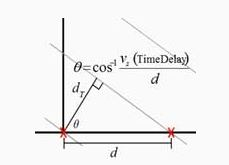
\includegraphics{figures/angle-of-arrival.jpg}
\caption{Angle of Arrival derivation ~\protect\cite{derivationSource}}
\label{fig:aoaDerivation}
\end{figure}

%This approach can be used for angle estimation from 0 to 180 degrees only and hence the application wouldn't be able to differentiate sound sources in first and third quadrants with same TDOA values. Similarly, it is not feasible to differentiate between sources in second and fourth quadrants with same values of TDOA. We believe that if a smartphone has a third microphone (many high end smartphones have 3 microphones), then we can remove this limitation and then this same approach can be used to detect angles from 0 to 360 degress.

\subsection{Display angle on UI}
Using the steps above, SoundDetector estimate angles to be displayed to the user. But before displaying, we need to apply a smoothing algorithm because sometimes temporary/sudden ambient noises causes interference leading to wrong angle prediction. So, it is important to minimize effects of these noises. Our smoothing algorithm is based on counting frequency of each estimated angle and then the final angle is the one with highest frequency. All estimated angles are recorded in a vector of length \textit{smoothing\_window} (equal to 10 in our experiments) and then the angle which was seen most frequently is displayed on the UI. Angle computation and display occurs on two separate threads. 
